\section{Experiments}
We evaluate \ours\ on both post-training and inference across LLM and agent settings. For post-training, we consider Logical Reasoning (LLM) and Multi-Hop Reasoning (Agent). For inference, we consider three representative open problem solving benchmarks: Circle Packing (Square), Circle Packing (Rectangle), and the Heilbronn Convex problem. In each benchmark, we compare \ours\ against commonly used baselines and show that \ours\ consistently achieves better sampling.

\subsection{Bidirectional Evolutionary Search for Post-Training}

\subsubsection{Logical Reasoning}
For logical reasoning, we use the Knights-and-Knaves dataset~\citep{kk}. In this task, each puzzle involves a group of people who are either a knight or a knave, and the solver must deduce each one's identity.

\begin{wrapfigure}{r}{0.45\textwidth}
\vspace{-1em}
\centering
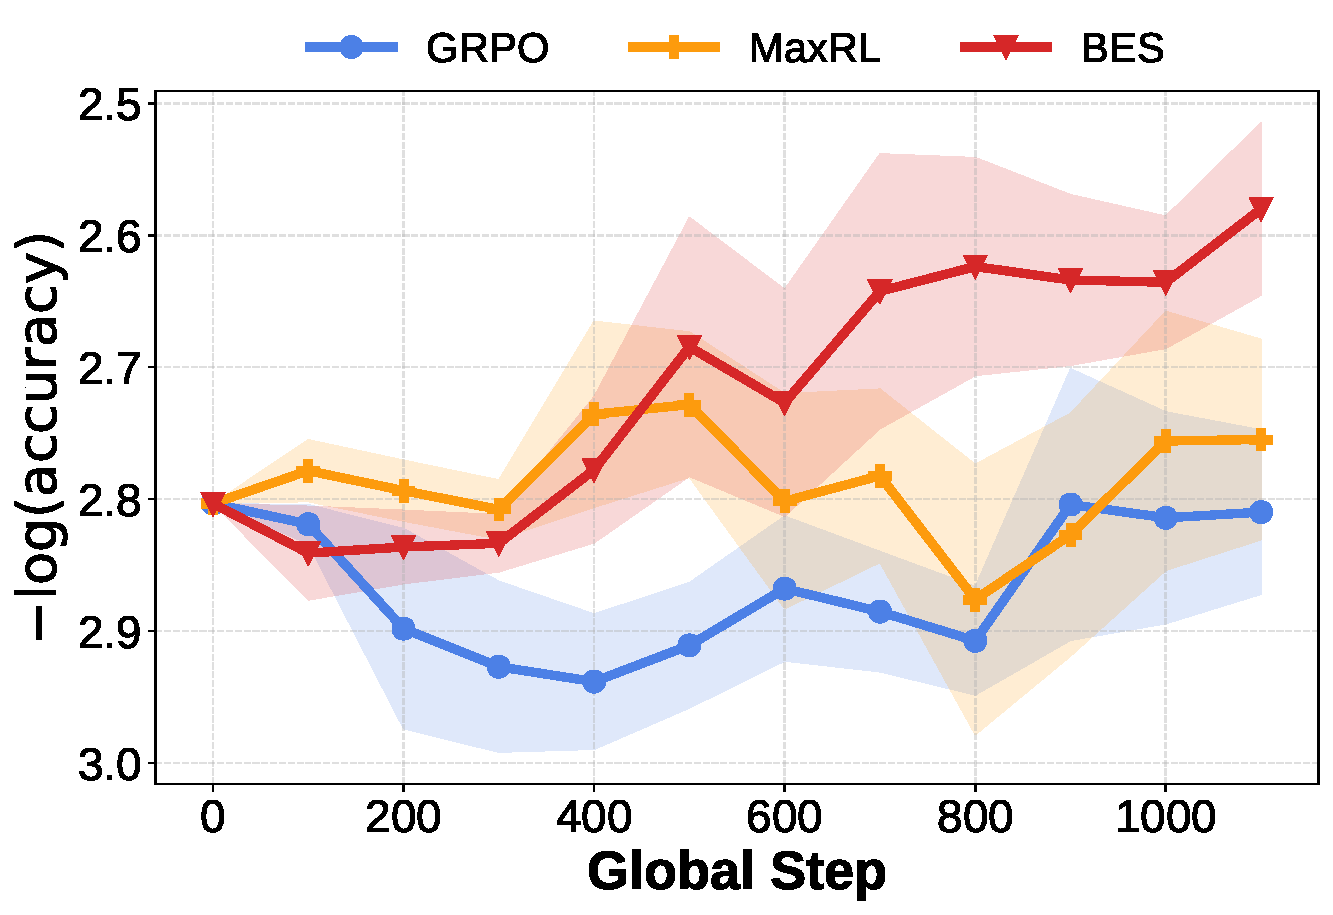
\includegraphics[width=0.43\textwidth]{images/bes_vs_baselines_overall.pdf}
\caption{EMA-smoothed validation accuracy on logical reasoning (Knights-and-Knaves).}
\label{fig:kk}
\vspace{-1em}
\end{wrapfigure}

\textbf{Baselines.} We select two post-training algorithms, GRPO~\citep{dsr1} and MaxRL~\citep{maxrl}, as baselines, as we apply \ours\ on top of MaxRL. We note that \ours\ is a sampling algorithm that is agnostic to the training method and can be applied on top of any post-training algorithm. 

\textbf{Training Setup.} We use Gemma-3-1B-it~\citep{gemma3} as the base model. 
To adapt the model to the Knights-and-Knaves benchmark, we first perform a cold start by fine-tuning on 1K SFT examples generated using the official data generation pipeline for 3 epochs, followed by 4 epochs of post-training on 5K problems, during which we compare the different methods on a 1.3K validation set. Detailed experimental configurations are provided in Appendix~\ref{app:logical_setup}. 

\textbf{Results.} As shown in Figure~\ref{fig:kk}, due to the difficulty of the training set, GRPO and MaxRL show little to no improvement during training, while \ours\ steadily improves on the validation set throughout training, demonstrating that \ours\ is more effective at discovering high-quality training samples.

\subsubsection{Multi-Hop Reasoning}



\begin{table*}[b]
\centering
\renewcommand{\arraystretch}{1.20}
\vspace{-1em}
\caption{Multi-hop reasoning post-training results on
MuSiQue with Llama-3.2-3B-Instruct and
Llama-3.1-8B-Instruct. We report accuracy, number of
valid searches, number of valid actions, and finish ratio. Higher is
better for all metrics. \textbf{Bold} denotes the best performing
method per backbone.}
\vspace{6pt}
\resizebox{\textwidth}{!}{%
\begin{tabular}{@{} l cccc @{}}
\toprule
\textbf{Method} 
& \textbf{Accuracy (\%, $\uparrow$)} 
& \textbf{\# Valid Search ($\uparrow$)} 
& \textbf{\# Valid Actions ($\uparrow$)} 
& \textbf{Finish Ratio ($\uparrow$)} \\
\midrule
\multicolumn{5}{@{}l}{\textit{Llama-3.2-3B-Instruct}} \\
\midrule[\lightrulewidth]
\rowcolor{cellbase}  Base model & 4.0 & -- & -- & -- \\
\rowcolor{cellbase}   + GRPO & 2.1 (-1.9) & 0.84 & 0.20 & 0.64 \\
\rowcolor{cellbase}  + Tree-GRPO & 3.9 (-0.1) & 1.50 & 2.14 & 0.64 \\
\rowcolor{tabband}   + \ours & \textbf{7.0 (+3.0)} & \textbf{2.31} & \textbf{3.29} & \textbf{0.97} \\
\midrule
\multicolumn{5}{@{}l}{\textit{Llama-3.1-8B-Instruct}} \\
\midrule[\lightrulewidth]
\rowcolor{cellbase}  Base model & 6.6 & -- & -- & -- \\
\rowcolor{cellbase}   + GRPO & 5.6 (-1.0) & 1.46 & 1.83 & 0.37 \\
\rowcolor{cellbase}  + Tree-GRPO & 7.4 (+0.8) & 0.65 & 1.36 & 0.71 \\
\rowcolor{tabband}   + \ours & \textbf{10.4 (+3.8)} & \textbf{2.11} & \textbf{3.05} & \textbf{0.94} \\
\bottomrule
\end{tabular}%
}
\label{tab:multihop}
\end{table*}

For multi-hop reasoning, we use the MuSiQue dataset~\citep{musique}. In this task, the agent must answer complex questions that require retrieving and integrating information across multiple documents, where no single document contains the complete answer. 

\textbf{Baselines.} We compare against GRPO~\citep{dsr1} and Tree-GRPO~\citep{treegrpo}, with the latter being the current state-of-the-art method for search agent post-training. We apply \ours\ on top of GRPO.

\textbf{Training Setup.} We adopt the training setup of Tree-GRPO~\citep{treegrpo}, using Llama-3.2-3B-Instruct and Llama-3.1-8B-Instruct~\citep{llama3} as base models. During the search process, the agent can perform multiple search actions before producing a final answer. Search results are provided by an offline Wikipedia server. We use the 3--4 hop solvable subset of the MuSiQue training set as our training data and train for 2 epochs, as additional epochs lead to training collapse. We evaluate on the full official MuSiQue validation set. Detailed configurations are provided in Appendix~\ref{app:qa_setup}.

\textbf{Results.} As shown in Table~\ref{tab:multihop}, GRPO consistently degrades from the base model on both scales, likely due to reward hacking where the model learns to skip search actions and guess directly, as reflected by its low number of valid searches. Tree-GRPO provides marginal improvement on the 8B model ($+0.8\%$) but fails to improve the 3B model. In contrast, \ours\ achieves substantial gains on both scales ($+3.0\%$ on 3B, $+3.8\%$ on 8B), outperforming all baselines by a wide margin. Beyond accuracy, \ours\ also produces agents with significantly more valid search actions and higher finish ratios, indicating that the trained agents learn to actively search rather than randomly guessing.



\subsection{Bidirectional Evolutionary Search for Inference}
At inference time, we evaluate the ability of \ours\ to solve open problems. Specifically, we consider three benchmarks: Circle Packing (Square), which seeks to pack $N$ circles into a unit square with maximum radius; Circle Packing (Rect), the analogous problem for a rectangular container; and Heilbronn (Convex), which seeks to place $N$ points in the unit square to maximize the minimum area of any convex polygon formed by subsets of the points.

\begin{table*}[h]
\centering
\vspace{-1em}
\renewcommand{\arraystretch}{1.20}
\caption{Open problem solving benchmarks with GPT-5 as the
backbone model. We report \textbf{Mean $\pm$ Std} and \textbf{Best}
objective values ($\uparrow$). \textbf{Bold} denotes the best
performing method.}
\vspace{6pt}
\resizebox{\textwidth}{!}{%
\begin{tabular}{@{} l cc cc cc @{}}
\toprule
\multirow{2}{*}{\textbf{Strategy}}
& \multicolumn{2}{c}{\textbf{Circle Packing (Square)}} 
& \multicolumn{2}{c}{\textbf{Circle Packing (Rect.)}} 
& \multicolumn{2}{c}{\textbf{Heilbronn (Convex)}} \\
\cmidrule(lr){2-3}
\cmidrule(lr){4-5}
\cmidrule(lr){6-7}
& Avg. & Best 
& Avg. & Best 
& Avg. & Best \\
\midrule
\multicolumn{7}{@{}l}{\textit{Human \& High-compute closed-source framework}} \\
\midrule[\lightrulewidth]
\rowcolor{cellbase} Human & -- & 2.634 & -- & 2.364 & -- & 0.0306 \\
\rowcolor{cellbase}  AlphaEvolve & -- & 2.635 & -- & 2.3658 & -- & 0.0309 \\
\midrule
\multicolumn{7}{@{}l}{\textit{Open-source frameworks}} \\
\midrule[\lightrulewidth]
\rowcolor{cellbase} OpenEvolve & 2.531 $\pm$ .018 & 2.541 & 2.267 $\pm$ .014 & 2.276 & 0.025 $\pm$ .005 & \textbf{0.027} \\
\rowcolor{cellbase}  GEPA & 2.613 $\pm$ .022 & 2.628 & 2.326 $\pm$ .023 & 2.354 & 0.025 $\pm$ .002 & \textbf{0.027} \\
\midrule
\multicolumn{7}{@{}l}{\textit{Base framework}} \\
\midrule[\lightrulewidth]
\rowcolor{cellbase} ShinkaEvolve & 2.464 $\pm$ .083 & 2.541 & 2.335 $\pm$ .026 & 2.358 & 0.023 $\pm$ .005 & 0.026 \\
\midrule
\multicolumn{7}{@{}l}{\textit{Ours}} \\
\midrule[\lightrulewidth]
\rowcolor{tabband}  \ours & \textbf{2.623} $\pm$ .014 & \textbf{2.632} & \textbf{2.349} $\pm$ .012 & \textbf{2.360} & \textbf{0.026} $\pm$ .001 & \textbf{0.027} \\
\bottomrule
\end{tabular}%
}
\label{tab:ops}
\end{table*}

\textbf{Baselines.} We compare against three open-source frameworks: OpenEvolve~\citep{openevolve}, GEPA~\citep{gepa}, and ShinkaEvolve~\citep{shinkaevolve}.  All baseline results are taken from SkyDiscover~\citep{skydiscover}, which uses the same backbone model, compute budget, and configuration as ours.  We apply \ours\ on top of ShinkaEvolve. For reference, we also include the results of human experts and AlphaEvolve~\citep{alphaevolve}, which is closed-source and uses significantly more compute than all other frameworks.

\textbf{Setup.} ShinkaEvolve maintains a population of candidate programs and iteratively proposes modifications. Since directly concatenating model outputs is not meaningful on this benchmark (where candidates are executable programs), we implement the evolution operators by prompting LLMs. We use GPT-5 as the backbone model. Detailed configurations are provided in Appendix~\ref{app:inference_setup}. 

\textbf{Results.} As shown in Table~\ref{tab:ops}, \ours\ outperforms open-source frameworks on every benchmark.  Notably, \ours\ also exhibits much lower variance across runs than all baselines, indicating the search is more stable and reliable. In Appendix~\ref{app:program}, we list a summary of the best programs discovered by \ours.




\subsection{Ablation Study}
\begin{wrapfigure}{r}{0.45\textwidth}
\vspace{-1em}
\centering
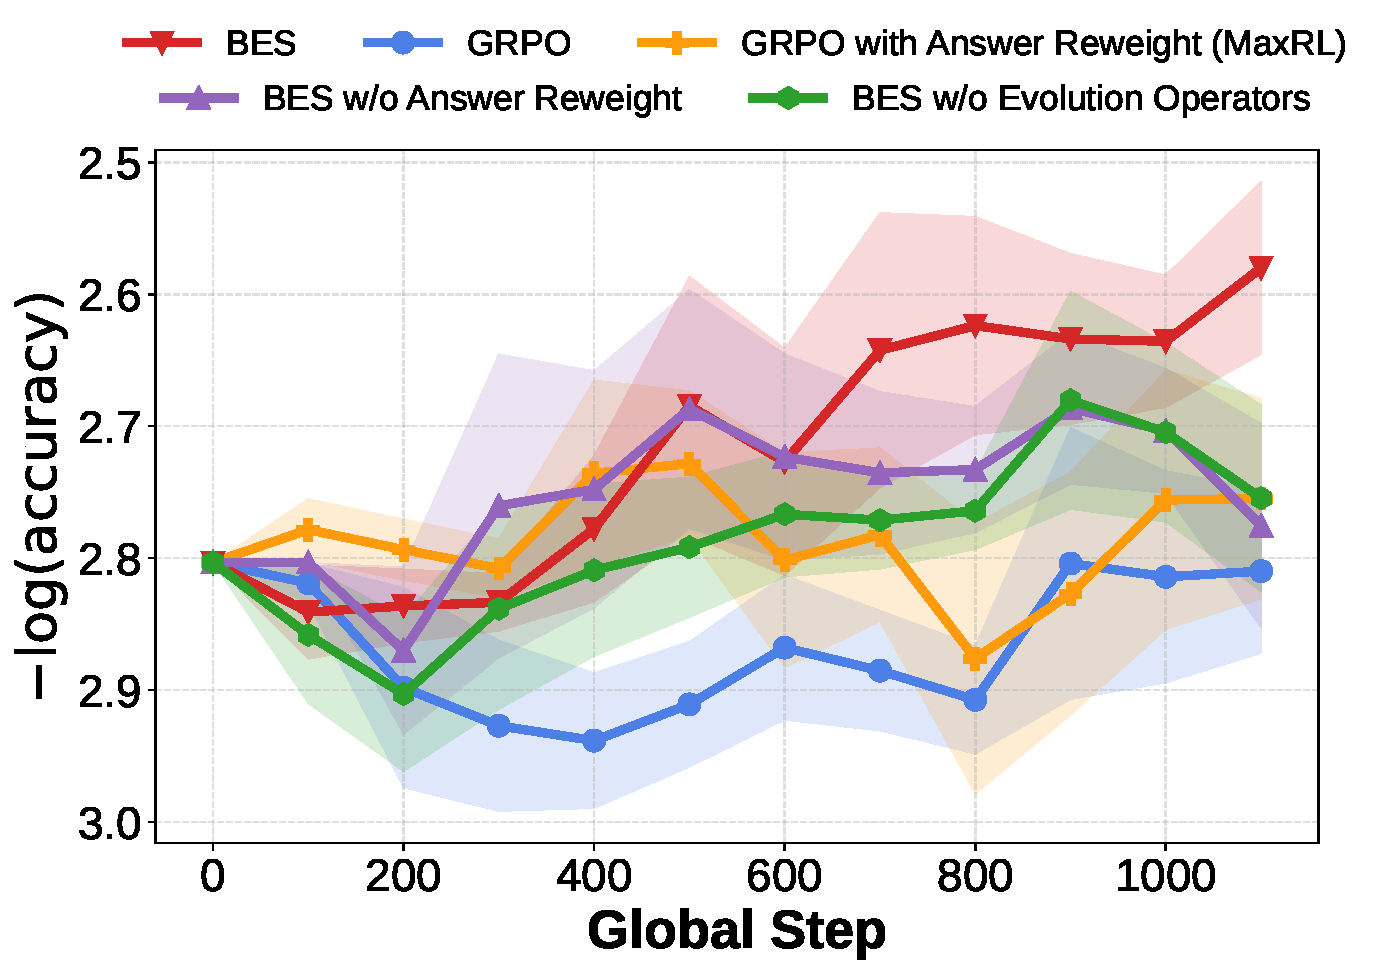
\includegraphics[width=0.43\textwidth]{images/bes_full_overall.pdf}
\vspace{-1em}
\caption{Ablation study on logical reasoning.}
\label{fig:kk_abl}
\vspace{-1em}
\end{wrapfigure}

We conduct an ablation study on the Knights-and-Knaves benchmark. On this benchmark, \ours\ combines bidirectional evolutionary search for discovering high-quality samples with MaxRL's answer reweighting for training. We therefore consider two ablations: (1) removing answer reweighting; and (2) removing the evolution operators to verify that both bidirectional search and evolution operators are necessary. As shown in Figure~\ref{fig:kk_abl}, both ablations underperform the full \ours\ method, while still outperforming the GRPO and MaxRL baselines. This confirms the effectiveness of each component in our approach.


\subsection{Cost Analysis}

\textbf{Post-Training.} To evaluate the cost-effectiveness of \ours, we compare the per-step wall-clock time and final accuracy across GRPO, Tree-GRPO, and \ours\ when training Llama-3.2-3B-Instruct on the agentic search task. We report the median wall-clock time per step throughout the training process.

\begin{table}[h]
\centering
\renewcommand{\arraystretch}{1.20}
\caption{Cost analysis for multi-hop reasoning post-training on Llama-3.2-3B-Instruct.}
\begin{tabular}{lccc}
\toprule
\textbf{Method} & \textbf{Accuracy (\%)} & \textbf{\# Valid Search} & \textbf{Walltime (s)} \\
\midrule
\rowcolor{cellbase} GRPO & 2.1 (-1.9) & 0.84 & 64 \\
\rowcolor{cellbase}  Tree-GRPO & 3.9 (-0.1) & 1.50 & 240 \\
\rowcolor{tabband} \ours & \textbf{7.0 (+3.0)} & \textbf{2.31} & 309 \\
\bottomrule
\end{tabular}
\label{tab:cost_posttraining}
\end{table}

Notably, the low wall-clock time of GRPO is misleading: during training, GRPO quickly exhibits reward hacking, with the model learning to skip search actions and guess answers directly, as reflected by its low number of valid searches. In contrast, \ours\ incurs less than 30\% additional overhead compared to Tree-GRPO, while achieving significantly better performance across all metrics.

\textbf{Inference.} We compare the API cost of \ours\ against ShinkaEvolve across all three open problem solving benchmarks. As shown in Table~\ref{tab:cost_inference}, \ours\ achieves consistently higher average values while incurring modest additional API costs.

\vspace{-0.5em}
\begin{table}[h]
\centering
\renewcommand{\arraystretch}{1.15}
\caption{Cost analysis for open problem solving. We report average API cost per generation.}
\begin{tabular}{lccccccccc}
\toprule
& \multicolumn{3}{c}{\textbf{Circle Packing (Sq.)}} & \multicolumn{3}{c}{\textbf{Circle Packing (Rect.)}} & \multicolumn{3}{c}{\textbf{Heilbronn (Convex)}} \\
\cmidrule(lr){2-4} \cmidrule(lr){5-7} \cmidrule(lr){8-10}
\textbf{Method} & Avg. & Best & Cost & Avg. & Best & Cost & Avg. & Best & Cost \\
\midrule
\rowcolor{cellbase} ShinkaEvolve & 2.464 & 2.541 & \$13.0 & 2.335 & 2.358 & \$11.9 & 0.023 & 0.026 & \$11.5 \\
\rowcolor{tabband} \ours & \textbf{2.623} & \textbf{2.632} & \$18.6 & \textbf{2.349} & \textbf{2.360} & \$14.0 & \textbf{0.026} & \textbf{0.027} & \$13.7 \\
\bottomrule
\end{tabular}
\label{tab:cost_inference}
\end{table}
\vspace{-1em}
